\documentclass{fizykalab}

% Ustawienia do tabelki

\wydzial{WI}
\autorjeden{Piotr Karamon}
\autordwa{Hubert Kasprzycki}
\rok{2}
\grupa{12}
\zespol{5}
\temat{Dyfrakcja światła na szczelinie pojedynczej i podwójnej}
\nrcwiczenia{71}
\datawykonania{17.10.2023}
\dataoddaniajeden{24.10.2023}
\zwrotdopoprawy{}
\dataoddaniadwa{}
\datazaliczenia{}

\usepackage{amsmath}
\usepackage{amsfonts}
\usepackage{parskip}

\newenvironment{conditions}[1][gdzie:]
  {#1 \begin{tabular}[t]{>{$}l<{$} @{${} - {}$} l}}
  {\end{tabular}\\[\belowdisplayskip]}

% \renewcommand{\arraystretch}{1.5}
\newcolumntype{L}[1]{>{\raggedright\let\newline\\\arraybackslash\hspace{0pt}}m{#1}}
\newcolumntype{C}[1]{>{\centering\let\newline\\\arraybackslash\hspace{0pt}}m{#1}}
\newcolumntype{R}[1]{>{\raggedleft\let\newline\\\arraybackslash\hspace{0pt}}m{#1}}

\usepackage[left=1.75cm, right=2cm, top=3cm]{geometry}
\usepackage[labelfont=bf]{caption}

\newcommand{\nm}{\ensuremath{\text{nm}}}
\newcommand{\mm}{\ensuremath{\text{mm}}}
\newcommand{\um}{\ensuremath{\mu \text{m}}}
\newcommand{\ju}{\ensuremath{\text{j.u.}}}


\usepackage{natbib}
\usepackage{url}
\begin{filecontents*}{test.bib}
@MISC{elportal-zlacze,
    author = {Michał Kurzela},
    title = {Dioda prostownicza - charakterystyka, oznaczenia, budowa},
    year = {2022},
    note = {[\url{https://elportal.pl/i/2022/09/06/12517-cfe4-1600x0_089-04.jpg}; odwiedzona  14.10.2023]},
    url = {https://elportal.pl/i/2022/09/06/12517-cfe4-1600x0_089-04.jpg}
}
\end{filecontents*}

\begin{document}

\maketitle

\section{Cel ćwiczenia}
Pomiar natężenia światła w obrazie dyfrakcyjnym pojedynczej szczeliny i układu dwu
szczelin. Wyznaczenie rozmiaru szczelin.

\section{Wstęp teoretyczny}
\subsection{Dyfrakcja na pojedynczej szczelinie}
Rozpatrujemy pojedynczą szczelinę o szerokości $a$.
W celu obliczenia natężenie promieniowania obserwowanego pod kątem $\theta$,
szczelina zostaje podzielona na dużą liczbę
odcinków, aby następnie zsumować pochodzące od nich fale cząstkowe.
Zakładamy, że rozmiar kątowy obrazu dyfrakcyjnego jest 
mały ($x << L$). Rozkład natężenie światła $I(x)$ wyraża się wzorem:
\begin{equation}
    I(x) = I_0
        {\left(
            \frac{sin\alpha}{\alpha}
        \right)}^2
    ,
    \quad \text{gdzie} \quad 
    \alpha = \frac{\pi a}{\lambda}\sin \theta \approx \frac{\pi a x}{\lambda L}
\end{equation}

\begin{conditions}
    \lambda  & długość fali świetlnej \\
    $L$ & odległość między szczeliną a ekranem
\end{conditions}


Własności obrazu dyfrakcyjnego dla pojedynczej szczeliny można 
wyprowadzić badając powyższą funkcję. Minima natężenia światła 
odpowiadają jej miejscom zerowym.

\begin{equation}
    \label{eq_x_min_dyfr}
    x_\text{min} = m\frac{\lambda L}{a}, \quad \text{gdzie} \quad
    m=\pm 1, \pm 2, \dots \quad \text{numer prążka dyfrakcyjnego} 
\end{equation}

W dobrym przybliżeniu maksima boczne odpowiadają maksimom funkcji 
$(\sin \alpha) ^2$, które można wyraźić wzorem:

\begin{equation}
    \label{eq_x_max_dyfr}
    x_\text{max} = \left(
        m + \frac{1}{2}
    \right)
    \frac{\lambda L}{a}
\end{equation}

\newpage
\subsection{Interferencja na dwóch szczelinach}
Dla układu dwóch szczelin ich szerokość a stanowi znaczą część odległości 
między nimi $d$. Rozkład natężenia jest złożeniem dyfrakcji oraz 
interferencji, przez co wyraża się wzorem.
\begin{equation}
    I(x) = I_0 {\left(
        \frac{\sin \alpha}{\alpha}
    \right)}^2 
    (\cos \beta)^2
    ,\quad \text{gdzie} \quad
    \alpha \approx \frac{\pi ax}{\lambda L},
    \quad \beta \approx \frac{\pi d x}{\lambda L}
\end{equation}

Prążki interferencyjne znajdują się w maksimach natężenia światła.
Ich umiejscowienie wyraża wzór
\begin{equation}
    \label{eq_x_max_interf}
    x_\text{max} = m \frac{\lambda L}{d}, \quad \text{gdzie} \quad m \in \mathbb{Z}
\end{equation}

Maksymalne natężenie światła w prążkach interferencyjnych nie jest stałe,
w przeciwieństwie do przypadku dwóch wąskich szczelin. Wynika to z występowania
zjawiska dyfrakcji, przez co niewielką liczbę najjaśniejszych prążków można 
zaobserwować w okolicach środkowego maksimum dyfrakcyjnego, w rejonach 
bocznych maksimów prążki te są ledwo widoczne.

\section{Aparatura pomiarowa}
W skład układu pomiarowego wchodziły następujące elementy:
\begin{enumerate}
    \item Laser czerwony o długości fali $\lambda = 650 \nm$
    \item Przesłona metalowa zawierająca: szczelinę pojedynczą oraz podwójną.
    \item Ekran zaopatrzony w fotodiodę, wraz z mechanizmem do jej przesuwania.
    \item Układ elektryczny do pomiaru odczytów fotodiody.
\end{enumerate}

\begin{figure}[H]
    \centering
    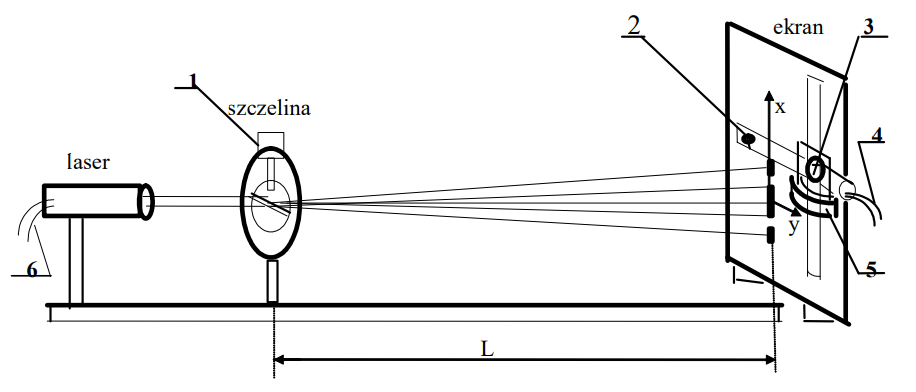
\includegraphics[width=1\linewidth]{uklad_pomiarowy.png}
    \caption{schemat układu pomiarowego}
    \label{fig:enter-label}
\end{figure}

\newpage
Układ elektryczny do pomiaru $I(x)$ składał się z następujących elementów:
\begin{enumerate}
    \item Fotodioda
    \item Woltomierz o pojedynczym zakresie pomiarowym 400 mV
    \item Bateria zasilająca $2 \times 1,5 \text{V}$
    \item Opornik regulowany dekadowy $10 \times 100 \Omega$
    \item Dodatkowe oporniki $1 \text{kV}$ i $2 \text{kV}$
\end{enumerate}

\begin{figure}[H]
    \centering
    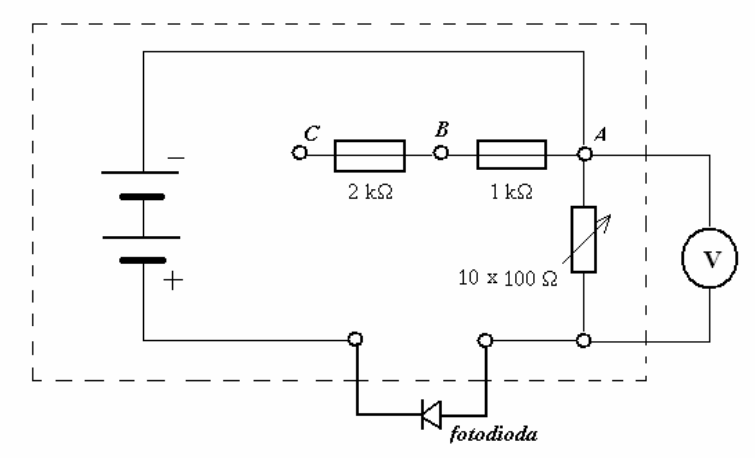
\includegraphics[width=0.75\linewidth]{uklad_elektryczny.png}
    \caption{schemat układu elektrycznego do pomiaru natężenia światłą}
    \label{fig:enter-label}
\end{figure}

\section{Przebieg doświadczenia}
\begin{enumerate}
    \item Na początku sprawdzono połączenie układu elektrycznego z fotodiodą.
    \item Fotodiodę ustawiona na maksimum główne, po czym zanotowano natężenie światła, jako wskazanie woltomierza.
    \item Diodę przesuwano w pionie, za każdym razem notując wskazania woltomierza.
    \item Laser wyłączono, a następnie zmierzono odległość szczeliny od ekranu.
\end{enumerate}
Doświadczenie zostało powtórzone dla układu dwóch szczelin.

\section{Wyniki pomiarów}

\subsection{Pojedyncza szczelina}

\begin{itemize}
    \item Odległość między szczeliną a ekranem $L = 673 \text{mm}$
    \item Długość fali $\lambda = 650 \text{nm}$
\end{itemize}


\begin{table}
    \centering
    \caption{Pomiary natężenia światła dla pojedynczej szczeliny.}
    \begin{tabular}{|c|c|}
        \hline
        \multicolumn{2}{|c|}{Wyniki w dół} \\ \hline
        \textbf{x [mm]} & \textbf{I [j.u.]} \\ \hline
        0 & 517 \\ \hline
        -0,2 & 465,8 \\ \hline
        -0,4 & 328,1 \\ \hline
        -0,6 & 200,5 \\ \hline
        -0,8 & 127,8 \\ \hline
        -1 & 96,1 \\ \hline
        -1,2 & 46,9 \\ \hline
        -1,4 & 29,5 \\ \hline
        -1,6 & 15,3 \\ \hline
        -1,8 & 12,9 \\ \hline
        -2 & 7 \\ \hline
        -2,2 & 5,1 \\ \hline
        -2,4 & 3,76 \\ \hline
        -2,6 & 3,57 \\ \hline
        -2,8 & 3,67 \\ \hline
        -3 & 3,22 \\ \hline
        -3,2 & 2,37 \\ \hline
        -3,4 & 1,93 \\ \hline
        -3,6 & 1,86 \\ \hline
        -3,8 & 1,68 \\ \hline
        -4 & 1,65 \\ \hline
        -4,2 & 1,12 \\ \hline
        -4,4 & 0,78 \\ \hline
        -4,6 & 0,43 \\ \hline
        -4,8 & 0,21 \\ \hline
        -5 & 0,19 \\ \hline
        -5,2 & 0,18 \\ \hline
        -5,4 & 0,15 \\ \hline
        -5,6 & 0,13 \\ \hline
        -5,8 & 0,07 \\ \hline
        -6 & 0,02 \\ \hline
        -6,2 & 0,03 \\ \hline
        -6,4 & 0,02 \\ \hline
        -6,6 & 0,03 \\ \hline
        -6,8 & 0,04 \\ \hline
        -7 & 0,05 \\ \hline
    \end{tabular}
    \quad
    \quad
    \begin{tabular}{|c|c|}
        \hline
        \multicolumn{2}{|c|}{Wyniki w górę} \\ \hline
        \textbf{x [mm]} & \textbf{I [j.u.]} \\ \hline
        0 & 517 \\ \hline
        0,2 & 377 \\ \hline
        0,4 & 214 \\ \hline
        0,6 & 102 \\ \hline
        0,8 & 46,4 \\ \hline
        1 & 24,5 \\ \hline
        1,2 & 11,4 \\ \hline
        1,4 & 7,2 \\ \hline
        1,6 & 4,7 \\ \hline
        1,8 & 3,83 \\ \hline
        2 & 3,41 \\ \hline
        2,2 & 2,53 \\ \hline
        2,4 & 1,95 \\ \hline
        2,6 & 1,36 \\ \hline
        2,8 & 0,97 \\ \hline
        3 & 0,76 \\ \hline
        3,2 & 0,7 \\ \hline
        3,4 & 0,6 \\ \hline
        3,6 & 0,6 \\ \hline
        3,8 & 0,53 \\ \hline
        4 & 0,4 \\ \hline
        4,2 & 0,23 \\ \hline
        4,4 & 0,15 \\ \hline
        4,6 & 0,12 \\ \hline
        4,8 & 0,11 \\ \hline
        5 & 0,11 \\ \hline
        5,2 & 0,08 \\ \hline
        5,4 & 0,05 \\ \hline
        5,6 & 0,04 \\ \hline
        5,8 & 0,04 \\ \hline
        6 & 0,04 \\ \hline
        6,2 & 0,06 \\ \hline
        6,4 & 0,07 \\ \hline
        6,6 & 0,07 \\ \hline
        6,8 & 0,06 \\ \hline
        7 & 0,05 \\ \hline
        7,2 & 0,08 \\ \hline
        7,4 & 0,09 \\ \hline
        7,6 & 0,1 \\ \hline
        7,8 & 0,09 \\ \hline
        8 & 0,05 \\ \hline
        8,2 & 0,04 \\ \hline
        8,4 & 0,04 \\ \hline
        8,6 & 0,04 \\ \hline
        8,8 & 0,04 \\ \hline
        9 & 0,04 \\ \hline
        9,2 & 0,04 \\ \hline
        9,4 & 0,03 \\ \hline
        9,6 & 0,02 \\ \hline
    \end{tabular}
\end{table}

\subsection{Podwójna szczelina}

\begin{itemize}
    \item Odległość między szczeliną a ekranem $L = 673 \text{mm}$
    \item Długość fali $\lambda = 650 \text{nm}$
\end{itemize}

\begin{table}[H]
    \centering
    \caption{Pomiary natężenie dla podwójnej szczeliny. Pomiary zostały wykonane
    niesymetrycznie, znacznie więcej pomiarów jest dla $x < 0$. Jest tak dlatego, że
    pomiary były wykonywane w bardzo ograniczonym czasie oraz w dużym pośpiechu.
    Gdy stwierdziliśmy, że wystarczy nam pomiarów dla $x > 0$ wróciliśmy do 
    położenia początkowego i  zbieraliśmy dane dla $x < 0$ do momentu 
    w którym nie skończył nam się czas.
    }
    \begin{tabular}{|c|c|}
        \hline
        \multicolumn{2}{|c|}{Wyniki w dół} \\ \hline
        \textbf{x [mm]} & \textbf{I [j.u.]} \\ \hline
        0 & 8,76 \\ \hline
        -0,1 & 8,3 \\ \hline
        -0,2 & 6,96 \\ \hline
        -0,3 & 5,3 \\ \hline
        -0,4 & 3,81 \\ \hline
        -0,5 & 2,48 \\ \hline
        -0,6 & 1,49 \\ \hline
        -0,7 & 1,05 \\ \hline
        -0,8 & 1,06 \\ \hline
        -0,9 & 1,55 \\ \hline
        -1 & 2,37 \\ \hline
        -1,1 & 3,43 \\ \hline
        -1,2 & 4,46 \\ \hline
        -1,3 & 5,29 \\ \hline
        -1,4 & 5,94 \\ \hline
        -1,5 & 5,13 \\ \hline
        -1,6 & 4,25 \\ \hline
        -1,7 & 3,04 \\ \hline
        -1,8 & 1,83 \\ \hline
        -1,9 & 1,04 \\ \hline
        -2 & 0,6 \\ \hline
        -2,1 & 0,47 \\ \hline
        -2,2 & 0,57 \\ \hline
        -2,3 & 0,91 \\ \hline
        -2,4 & 1,38 \\ \hline
        -2,5 & 2,02 \\ \hline
        -2,6 & 2,52 \\ \hline
        -2,7 & 2,73 \\ \hline
        -2,8 & 2,57 \\ \hline
        -2,9 & 2,17 \\ \hline
        
    \end{tabular}
    \begin{tabular}{|c|c|}
        \hline
        \textbf{x [mm]} & \textbf{I [j.u.]} \\ \hline
        
        -3 & 1,64 \\ \hline
        -3,1 & 1,21 \\ \hline
        -3,2 & 0,84 \\ \hline
        -3,3 & 0,58 \\ \hline
        -3,4 & 0,38 \\ \hline
        -3,5 & 0,23 \\ \hline
        -3,6 & 0,2 \\ \hline
        -3,7 & 0,2 \\ \hline
        -3,8 & 0,31 \\ \hline
        -3,9 & 0,4 \\ \hline
        -4 & 0,51 \\ \hline
        -4,1 & 0,56 \\ \hline
        -4,2 & 0,58 \\ \hline
        -4,3 & 0,62 \\ \hline
        -4,4 & 0,59 \\ \hline
        -4,5 & 0,5 \\ \hline
        -4,6 & 0,36 \\ \hline
        -4,7 & 0,24 \\ \hline
        -4,8 & 0,12 \\ \hline
        -4,9 & 0,06 \\ \hline
        -5 & 0,02 \\ \hline
        -5,1 & 0,01 \\ \hline
        -5,2 & 0,02 \\ \hline
        -5,3 & 0,02 \\ \hline
        -5,4 & 0,01 \\ \hline
        -5,5 & 0,02 \\ \hline
        -5,6 & 0,02 \\ \hline
        -5,7 & 0,02 \\ \hline
    \end{tabular}
    \quad
    \quad
    \begin{tabular}{|c|c|}
        \hline
        \multicolumn{2}{|c|}{Wyniki w górę} \\ \hline
        \textbf{x [mm]} & \textbf{I [j.u.]} \\ \hline
        0 & 8,76 \\ \hline
        0,1 & 8,11 \\ \hline
        0,2 & 6,71 \\ \hline
        0,3 & 5,2 \\ \hline
        0,4 & 3,57 \\ \hline
        0,5 & 2,37 \\ \hline
        0,6 & 1,57 \\ \hline
        0,7 & 1,2 \\ \hline
        0,8 & 1,31 \\ \hline
        0,9 & 1,93 \\ \hline
        1 & 2,94 \\ \hline
        1,1 & 4,17 \\ \hline
        1,2 & 5 \\ \hline
        1,3 & 5,3 \\ \hline
        1,4 & 5,45 \\ \hline
        1,5 & 5,4 \\ \hline
        1,6 & 4,98 \\ \hline
        1,7 & 4 \\ \hline
        1,8 & 3,17 \\ \hline
        1,9 & 2,34 \\ \hline
        2 & 1,57 \\ \hline
        2,1 & 1,94 \\ \hline
        2,2 & 0,67 \\ \hline
        2,3 & 0,71 \\ \hline
        2,4 & 0,99 \\ \hline
        2,5 & 1,54 \\ \hline
        2,6 & 2,14 \\ \hline
        2,7 & 2,82 \\ \hline
        2,8 & 3,33 \\ \hline
        2,9 & 3,62 \\ \hline
        3 & 3,6 \\ \hline
        3,1 & 2,93 \\ \hline
        3,2 & 2,1 \\ \hline
        3,3 & 1,32 \\ \hline
    \end{tabular}
\end{table}

\section{Opracowanie wyników}

\subsection{Pojedyncza szczelina}

\begin{figure}[H]
    \centering
    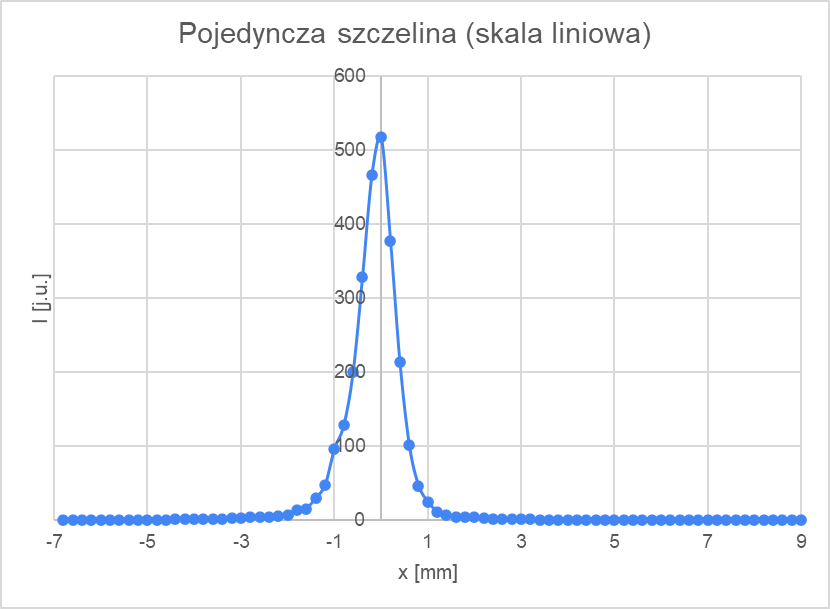
\includegraphics[width=0.65\linewidth]{wykres_poj_lin.png}
    \caption{Pomiary natężenia światła dla szczeliny pojedynczej w skali liniowej.}
\end{figure}

\begin{figure}[H]
    \centering
    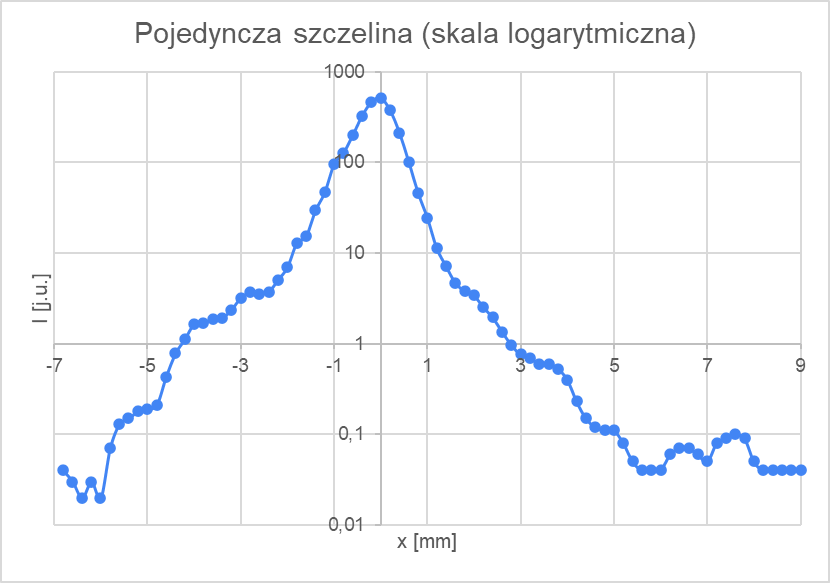
\includegraphics[width=0.65\linewidth]{wykres-poj-log.png}
    \caption{Pomiary natężenia światła dla szczeliny pojedynczej w skali logarytmicznej.
    }
\end{figure}

Uzyskany wykres w bardzo znacznym stopniu odbiega od wykresu teoretycznego.
Istnieje kilka możliwych powodów 
dlaczego wykres nie jest zgodny z wykresem teoretycznym:
\begin{itemize}
    \item Efekty otoczenia: Zanieczyszczenia powietrza, 
    może wpłynąć na wyniki dyfrakcji i doprowadzić do nieprawidłowych wykresów.
    \item Źle skonfigurowany woltomierz, którego odczyt służył za miarę
          intensywności światła.
    \item Błędy ze strony ludzkiej, złe spisanie pomiarów, pomyłki 
          w procesie przesuwania fotodiody w pionie, 
          dobranie złego zakresu na woltomierzu.
    \item Sama szczelina przez którą przepuszczane było światło,
          która mogła być uszkodzona.
    \item Złe ustawienie samej szczeliny w stosunku do ekranu,
          przez co jakość uzyskanego obrazu była zbyt słaba.
\end{itemize}

\begin{table}[H]
    \centering
    \caption{Położenia maksimów i minimów natężenia światła dla 
    pojedynczej szczeliny
    }
    \begin{tabular}{|C{3.5cm}|C{2cm} | C{2cm}| C{2cm} |C{2cm}|}
        \hline
         Element obrazu dyfrakcyjnego&
         Położenie z lewej $x_l$ [mm]&
         Położenie z prawej $x_p$ [mm]& 
         $x = \frac{x_p - x_l}{2}$ [mm]& 
         Obliczona szerokość szczeliny $a$ [mm]
         
         \\ \hline
         1 minimum  &
         -2,6 & 1,8 & 2,2 & 0,198840 \\ \hline
         1 maksimum boczne &
         -2,8 & 2 & 2,4 & 0,273406\\ \hline
         2 minimum &
         -3,4 & 3 & 3,2 & 0,273406 \\ \hline
         2 maksimum boczne&
         
         -4 & 3,6 & 3,8 & 0,287796 \\ \hline
    \end{tabular}
    \label{tab:my_label}
\end{table}

Korzystając ze zmierzonych minimów oraz wzoru (\ref{eq_x_min_dyfr}) wyznaczamy wzór na 
szerokość pojedynczej szczeliny $a$:

\begin{equation}
    a = \frac{m \lambda L} {x_\text{min}}
\end{equation}

\begin{align*}
    a_1 &= \frac{1 \cdot 650 \nm  \cdot 673 \mm}{2,2 \mm} = 198,840 \um \\
    a_2 &= \frac{2 \cdot 650 \nm  \cdot 673 \mm}{3,2 \mm} = 273,406 \um \\
\end{align*}

Tym razem korzystając ze zmierzonych maksimów oraz wzoru (\ref{eq_x_max_dyfr}) wyznaczamy wzór na 
szerokość pojedynczej szczeliny $a$:

\begin{equation}
    a = \left(m + \frac{1}{2}\right) \frac{\lambda L} {x_\text{max}}
\end{equation}

\begin{align*}
    a_3 &= \left(1 + \frac{1}{2}\right) \frac{650 \nm \cdot 673 \mm} {2,4 \mm} = 273,406 \um \\
    a_4 &= \left(2 + \frac{1}{2}\right) \frac{650 \nm \cdot 673 \mm} {3,8 \mm} = 287,796 \um \\
\end{align*}

Obliczamy wartość średnią $a$.

\begin{equation*}
    \overline{a} = \frac{a_1 + a_2 + a_3 + a_4}{4} = \frac{198,840 \um +  273,406 \um +  273,406 \um + 287,796 \um}{4} = 258,362 \um
\end{equation*} 

Aby uzyskać niepewność pomiarową $\overline{a}$ użyjemy odchylenia standardowego
(nie odchylenia standardowego średniej, ponieważ ilość pomiarów jest mała).

\begin{equation*}
    u(\overline{a}) = \sqrt{
         \frac{
             \left(a_1- \overline{a} \right)^2 + 
             \left(a_2- \overline{a} \right)^2 + 
             \left(a_3- \overline{a} \right)^2 +
             \left(a_4- \overline{a} \right)^2
         }{4-1}} =  
         \sqrt{\frac{
             \begin{aligned}\left(198,840 \um - 258,362 \um \right)^2 &+ \\
             \left(273,406 \um - 258,362 \um \right)^2 &+  \\
             \left(273,406 \um - 258,362\um \right)^2  &+  \\
             \left(287,796 \um - 258,362\um \right)^2\end{aligned}
         }{4-1}} =  35 \um
\end{equation*}

Zatem niepewność rozszerzona $U(\overline{a}) = 2\cdot u(\overline{a}) = 70 \um$
Ostatecznie możemy zapisać 

\begin{equation*}
    a = 258\um \pm 70\um 
\end{equation*}

Jak widać niepewność naszego pomiaru jest wysoka, czego można się było 
spodziewać zważywszy na to jak bardzo nasz wykres odbiega od wykresu 
teoretycznego. 
\begin{table}[H]
    \centering
    \caption{Natężenia światła w maksimach bocznych. Natężenie światła w maksimum głównym:
        $I_o = 517 [\text{j.u.}]$
    }
    \begin{tabular}{|C{3.5cm}|C{2cm} | C{2cm}| C{2.5cm} |C{2cm}|}
        \hline
         Element obrazu dyfrakcyjnego&
         Natężenie z lewej $I_l$ [j.u.]&
         Natężenie z prawej $I_p$ [j.u.]& 
         Natężenie względne doświadczalne
         $\frac{I(x_\text{max})}{I_o} = \frac{I_l + I_p}{2I_0}$
         & 
         Natężenie względne teoretyczne  $\frac{I(x_\text{max})}{I_0}$ 
         
         \\ \hline
         1 maksimum boczne &
         3.67 & 3.41 & 0,00684 & 0,045 \\ \hline
         2 maksimum boczne&
         
         1.65 & 0.6 & 0,00217 & 0,0162 \\ \hline
    \end{tabular}
\end{table}

Obliczamy natężenie względne teoretyczne korzystając ze wzoru

\begin{equation*}
    \frac{I(x_\text{max})}{I_0} \approx \frac{1}{\pi^2 (m + \frac{1}{2})^2}
\end{equation*}

Dla 1 maksimum bocznego:
\begin{align*}
    \text{wartość doświadczalna  } \quad &\frac{I(x_\text{max})}{I_0} = \frac{3,67 \ju + 3,41 \ju}{2 \cdot 517 \ju} = 0,00684 \\
    \text{wartość teoretyczna  } \quad &\frac{I(x_\text{max})}{I_0} \approx \frac{1}{\pi^2 (1 + \frac{1}{2})^2} = 0,045
\end{align*}

Dla 2 maksimum bocznego:
\begin{align*}
    \text{wartość doświadczalna  } \quad & \frac{I(x_\text{max})}{I_0} = \frac{3,67 \ju + 3,41 \ju}{2 \cdot 517 \ju} = 0,00217 \\
    \text{wartość teoretyczna  } \quad & \frac{I(x_\text{max})}{I_0} \approx \frac{1}{\pi^2 (2 + \frac{1}{2})^2} = 0,0162
\end{align*}

Dla obu maksimów wartość natężenia wynikająca z pomiarów wyszła kilkukrotnie mniejsza niż wartość wyliczona teoretycznie. Spowodowane jest to jak już wcześniej wspomnianym odbieganiem naszego wykresu od wykresu teoretycznego.

\subsection{Podwójna szczelina}

\begin{figure}[H]
    \centering
    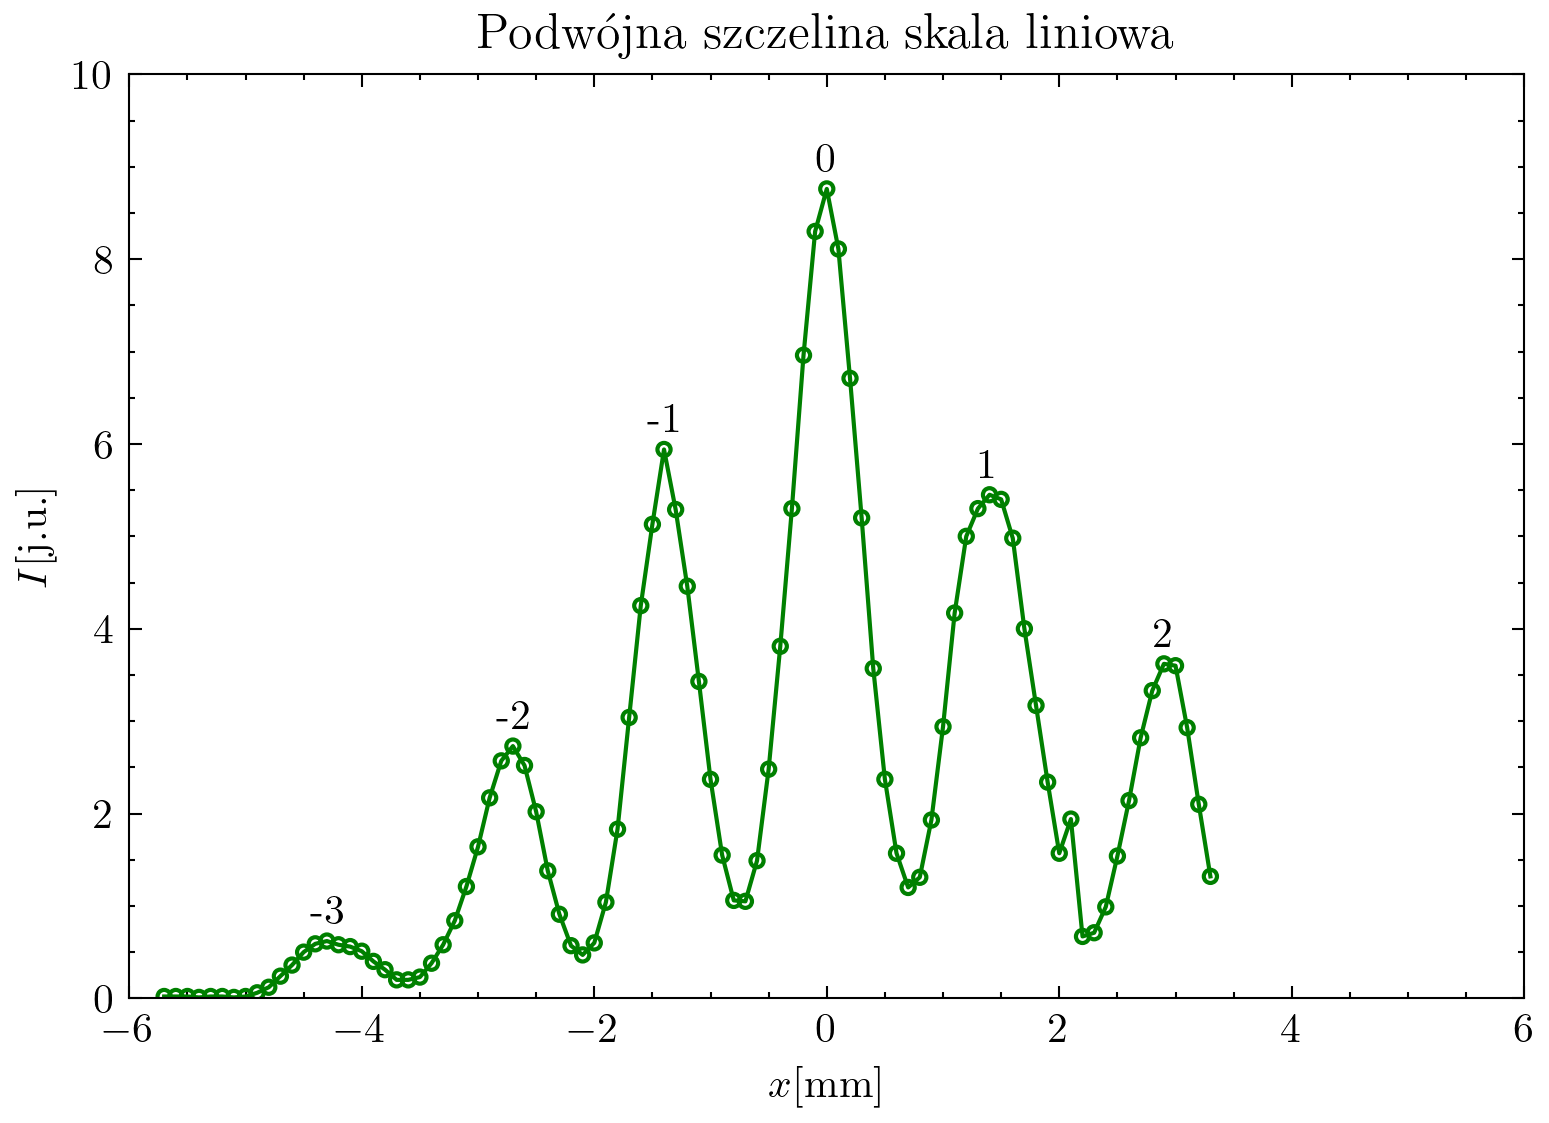
\includegraphics[width=0.65\linewidth]{powdojna_liniowa_numery_maksimum.png}
    \caption{Pomiary natężenia światła dla szczeliny podwójnej w skali liniowej.
    Na wykresie poza punktami pomiarowymi oraz gładką krzywą znajdują się liczby
    całkowite $-3, -2, -1, 0, 1, 2$ które oznaczają numery maksimów.
    }
\end{figure}

% \begin{figure}[H]
%     \centering
%     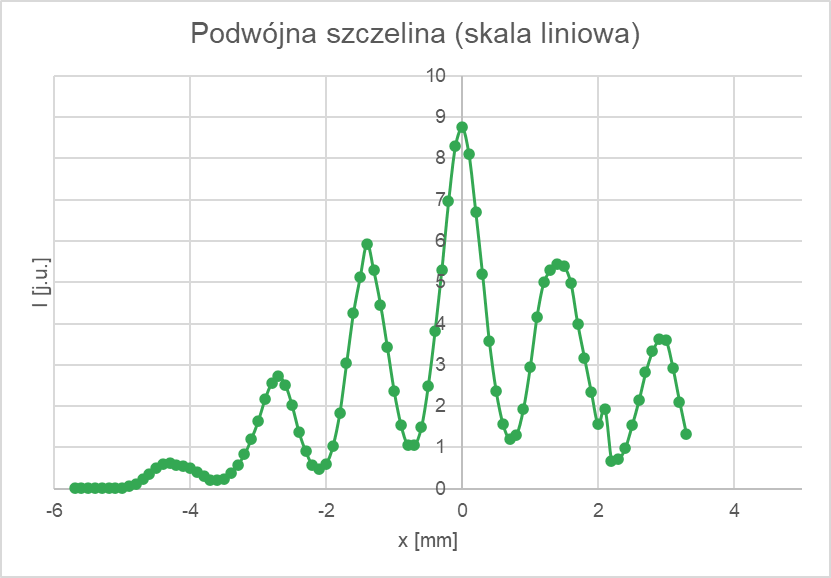
\includegraphics[width=0.5\linewidth]{wykres-podw-lin.png}
% \end{figure}

% \begin{figure}[H]
%     \centering
%     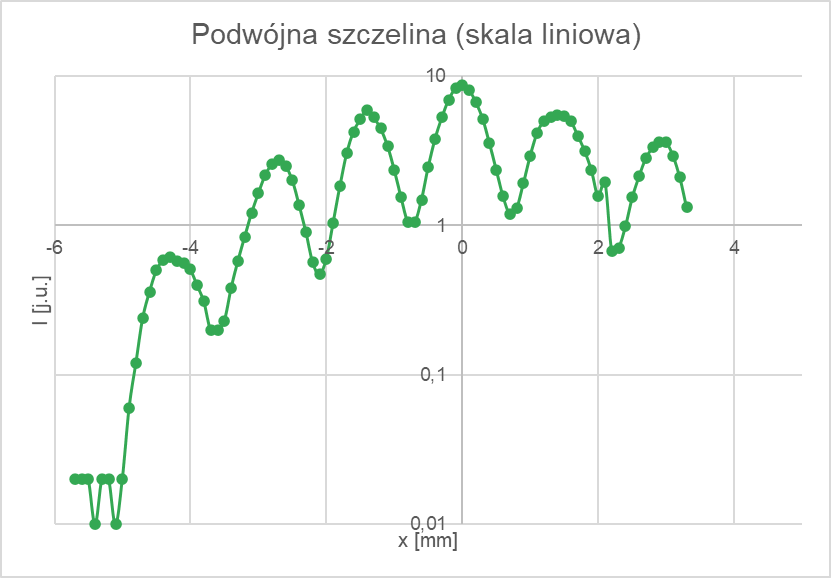
\includegraphics[width=0.5\linewidth]{wykres-podw-log.png}
% \end{figure}

\begin{table}[H]
    \centering
    \caption{Położenia maksimów  natężenia światła dla 
    podwójnej szczeliny.
    }
    \begin{tabular}{|C{2cm}|C{2cm} | C{2cm}| C{2cm} |C{2cm}|}
        \hline
         Numer maksimum $|m|$ &
         Położenie z lewej $x_l$ [mm]&
         Położenie z prawej $x_p$ [mm]& 
         $x = \frac{x_p - x_l}{2}$ [mm]& 
         Obliczona odległość $d$ [mm]
         \\ \hline
         1 & -1,4 & 1,4 & 1,4 & 0,312  \\ \hline
         2 & -2,7 & 2,9 & 2,8 & 0,312 \\ \hline
         3 & -4,3 & brak danych & 4,3 & 0,305 \\ \hline
    \end{tabular}
    \label{tab:my_label}
\end{table}

Korzystając ze wzoru (\ref{eq_x_max_interf}) wyznaczamy wzór na 
odległość między szczelinami $d$:

\begin{equation}
    d = \frac{m \lambda L} {x_\text{max}}
\end{equation}

\begin{align*}
    d_1 &= \frac{1 \cdot 650 \nm  \cdot 673 \mm}{1.4 \mm} = 312,4643 \um \\
    d_2 &= \frac{2 \cdot 650 \nm  \cdot 673 \mm}{2.8 \mm} = 312,4643 \um \\
    d_3 &= \frac{3 \cdot 650 \nm  \cdot 673 \mm}{4.3 \mm} = 305,1977 \um \\
\end{align*}

 
Obliczamy wartość średnią $d$.

\begin{equation*}
    \overline{d} = \frac{d_1 + d_2 + d_3}{3} = \frac{312,4643 \um +  312,4643 \um +  305,1977 \um}{3} = 310,0421 \um
\end{equation*} 

Aby uzyskać niepewność pomiarową $\overline{d}$ użyjemy odchylenia standardowego
(nie odchylenia standardowego średniej, ponieważ ilość pomiarów jest mała).

\begin{multline*}
    u(\overline{d}) = \sqrt{
         \frac{
             \left(d_1- \overline{d} \right)^2 + 
             \left(d_2- \overline{d} \right)^2 + 
             \left(d_3- \overline{d} \right)^2 
         }{3-1}} = \\ = 
         \sqrt{\frac{
             \left(312,4643 \um - 310,0421 \um \right)^2 + 
             \left(312,4643 \um - 310,0421 \um \right)^2 + 
             \left(305,1977 \um - 310,0421\um \right)^2 
         }{3-1}} = 4,2 \um
\end{multline*}

Zatem niepewność rozszerzona $U(\overline{d}) = 2\cdot u(\overline{d}) = 8,4 \um$
Ostatecznie możemy zapisać 

\begin{equation*}
    d = 310,0\um \pm 8,4\um 
\end{equation*}


Dla $x = 0$ osiągane jest natężenie maksymalne równe $I_\text{max} = 8,76 \ju$
Najbliższe $x=0$ minimum znajduję się w $x = 0.7 \mm$ jest ono równe
$I_\text{min} = 1,20 \ju$. Stosunek tych wartości jest równy:

\begin{equation*}
\frac{I_\text{min}}{I_\text{max}} = \frac{1,20 \ju}{8,76 \ju} = 0,137
\end{equation*}

Ta wartość jest miarą jakości obrazu interferencyjnego. Dla obrazu idealnego 
$I_\text{min} / I_\text{max} = 0$, natomiast wartość  $I_\text{min} / I_\text{max} = 1$
oznacza zniknięcie prążków interferencyjnych.
Otrzymana przez nas wartość zawiera się w przedziale $(0,1)$ oraz jest bliska wartości $0$,
co oznacza, że jakość obrazu interferencyjnego była dość wysoka.




\section{Wnioski}
\begin{enumerate}
    \item Światło istotnie ma charakter falowy,
          ponieważ ulega zjawiskom dyfrakcji i interferencji.
    \item Przy przepuszczaniu przez dwie szczeliny następują dwa zjawiska na
            raz – dyfrakcja i interferencja, przez co obraz tworzy serię kropek o
            różnych natężeniach.
    \item Nasze pomiary oraz obliczenia związane z pojedynczą szczeliną zdecydowanie
          nie są zbyt zadowalające. Może być to spowodowane złą 
          konfiguracją sprzętu pomiarowego m.in: lasera, szczeliny, układu do pomiaru
          natężenia światła. Warto również wspomnieć, iż przy wyprowadzaniu
          wzorów teoretycznych popełniane są pewne założenia, które nie konieczne 
          mogły być prawdziwe w momencie gdy robiliśmy doświadczenie.
    \item Wykres oraz obliczone wartości dla szczeliny  podwójnej były już o
    wiele bardziej zadowalające. Udało nam się uzyskać wykres
    $I_\text{światła} = f(x)$ który jest zgodny z teorią. Wyliczona odległość 
    między szczeliną oraz jej niepewność
    wydają się być sensowne. Przeprowadzone przez nas doświadczenie 
    ukazuje falowy charakter światła, ponieważ jak każda inna fala
    ulega ono zjawisku dyfrakcji i interferencji.
    \item 
    Choć wykres $I_\text{światła} = f(x)$ jest podobny do teoretycznego to nadal
    trochę się od niego różni z  kilku powodów:
        \begin{itemize}
            \item Detektor natężenia światła uśrednia funkcję $I(x)$ 
            na obszarze, z którego pobiera informacje,
            \item  W wyniku czego natężenie w maksimach ulega obniżeniu,
                   a w minimach natężenie jest większe od 0.
            \item  Szczelina może być nierówna, a wiązka laserowa nie
            jest  zupełnie równoległa.
        \end{itemize}
        
\end{enumerate}


% \renewcommand{\refname}{Bibliografia}
% \bibliographystyle{alpha}
% \bibliography{test}
\end{document}